
\documentclass{article}

\usepackage[utf8]{inputenc}
\usepackage[left=1.5in,right=1.5in,bottom=1in]{geometry}
 \usepackage{setspace} \onehalfspacing
\setlength\parindent{0pt}
\setlength{\parskip}{1em}
\setcounter{secnumdepth}{0}
\usepackage{outlines}
\usepackage{graphicx}
\usepackage{caption}
\graphicspath{ {imgs} }
\usepackage{hyperref}
\usepackage{enumerate}


\usepackage[
backend=biber,
style=alphabetic,
sorting=ynt
]{biblatex}
\addbibresource{photo_essay.bib}

\title{Ninoofsepoort Park, Molenbeek, and `The Triangle'}
\author{Carla Hyenne}

\begin{document}

\maketitle

\begin{figure}[h!]
	\centering
	\captionsetup{labelformat=empty}
	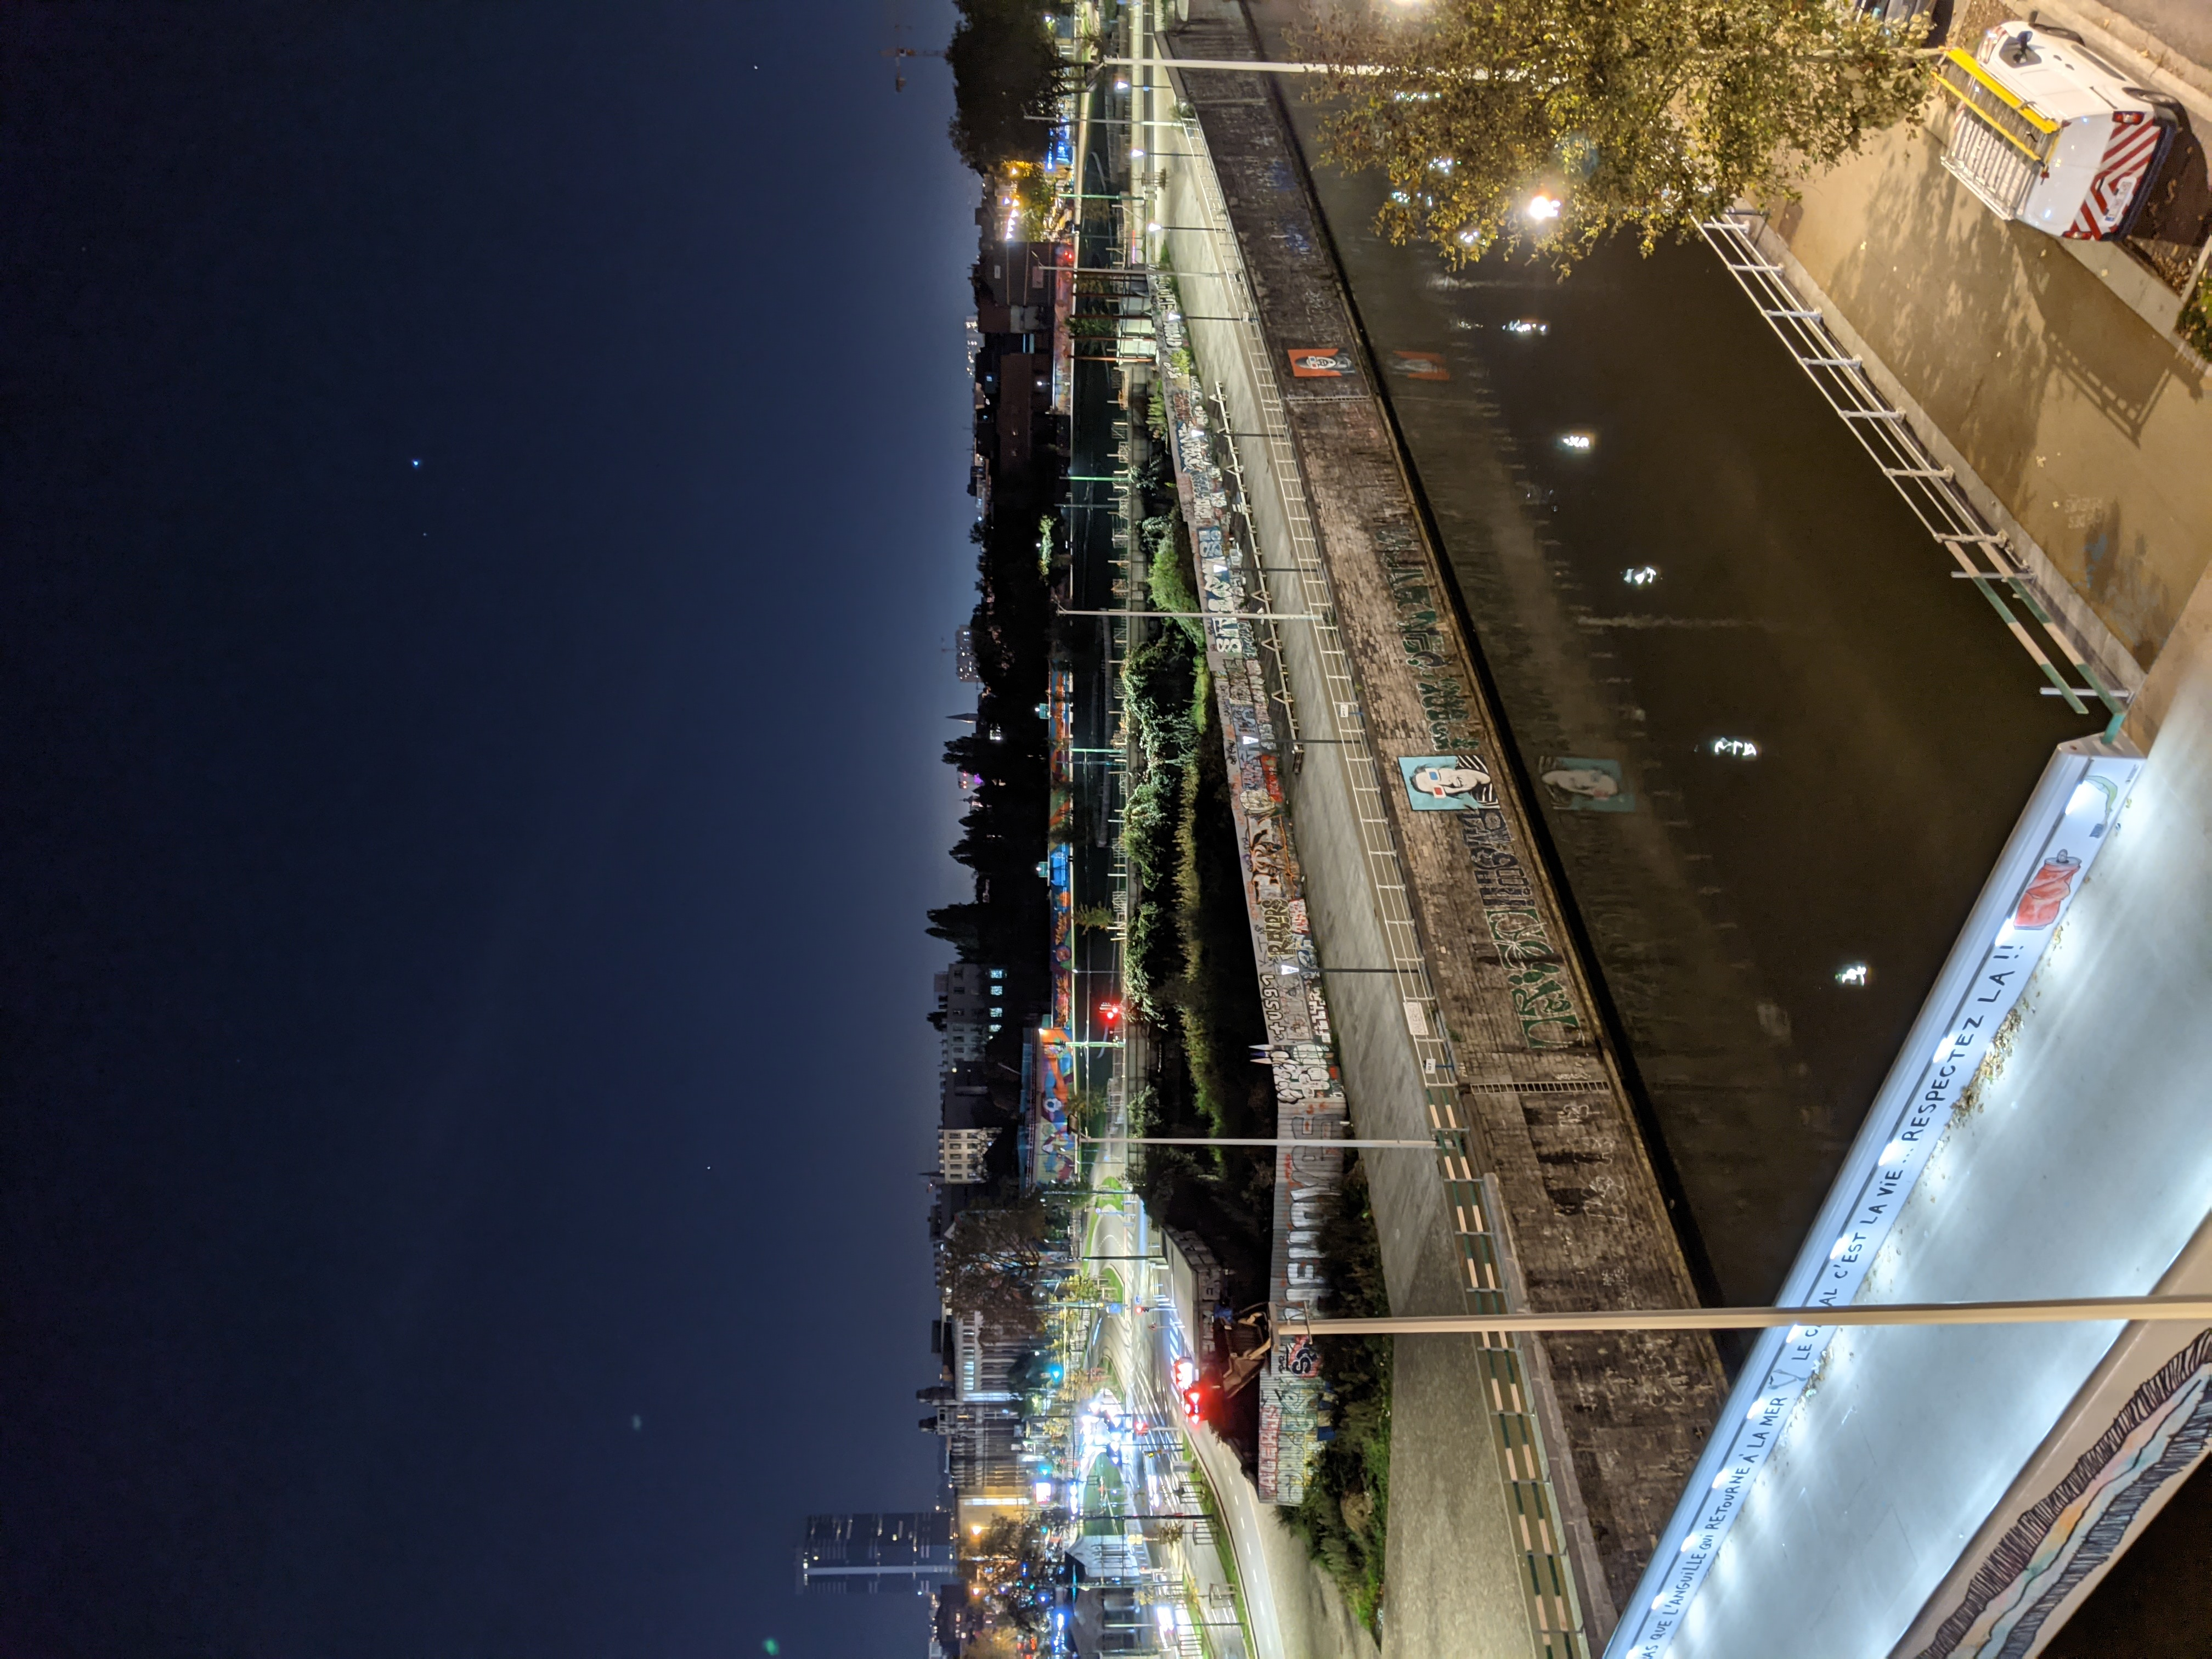
\includegraphics[width=\textwidth, angle=-90]{bxl_canal_far}
	\caption{View towards the Ninoofsepoort park from the rooftop of the MIMA museum, Sint-Jans-Molenbeek, October 23rd 2021}
\end{figure}

\pagebreak


\begin{enumerate}
	\item Ninoofsepoort park was developed in ????. There was considerable debate about what to do with this space\marginpar{what else was being considered?}.
	\item Viewed from above, it looks like another park sits between the canal and Ninoofseport park. It lush, overgrown greenery, but is surrounded by a wooden fence covered in graffiti 
	\item Size and potential for the site: it's triangular, not very big\marginpar{Can I get measurements?}. Given the size and location constraints, what could it be?
	\item What existing proposals are there for this site?
	\item What actors are at play here?
	\item We can also notice the canal art: two faces looking at us with 3D glasses. This is a satirical piece by ????, to provoke reflection around people coming in 2016 to observe Molenbeek as a ``breeding site for terrorists''. The city of Brussels' plan for the (re)development of the canal, which will inevitably influence Molenbeek, is quite in contrast with tis view of an unsafe, sketchy neigbhourhood.
	\item Once the development is completed, this view will most likely not exist. A building will stand in the way, and will most likely be as tall as regulations allow\marginpar{what building will it be? what's the height limit for brussels?}
	
\end{enumerate}

- relate to lecture 5, and gentrification: using MIMA as a regeneration project, near the new centre pompidou,


\pagebreak

\printbibliography 

\end{document}
